\chapter{Simplex - Matrix Calculations}

\section{Solutions to $A\x = \b$}
\begin{outcome}
\begin{itemize}
\item Explore how a system of equations can be rewritten via partitioning the variables
\item See how we can also partition the matrix and rewrite the equation in a new format that solves for basic variables
\item Familiarize with matrix notation
\item Define terminology of a basic solution and a basic feasible solution
\end{itemize}
\end{outcome}
We will now explore ways to represent solutions to this linear system of equations.  This is meant to give the theoretical backbone of the simplex algorithm.  

We consider a linear system

$$
A \mathbf{x} = \mathbf{b},
$$

where $A \in \mathbb{R}^{m \times n}$, $\mathbf{x} \in \mathbb{R}^n$, and $\mathbf{b} \in \mathbb{R}^m$. Explicitly,

$$
A =
\begin{bmatrix}
    a_{11} & \cdots & a_{1n} \\
    \vdots & \ddots & \vdots \\
    a_{m1} & \cdots & a_{mn}
\end{bmatrix}, \quad
\mathbf{x} =
\begin{bmatrix}
    x_1 \\
    \vdots \\
    x_n
\end{bmatrix}, \quad
\mathbf{b} =
\begin{bmatrix}
    b_1 \\
    \vdots \\
    b_m
\end{bmatrix}.
$$

\subsection*{Assumptions on $A$}

We assume:
\begin{itemize}
\item $\text{rank}(A) = m$, i.e., the rows of $A$ are linearly independent (full row rank);
\item $m \leq n$, so the system is not overdetermined.
\end{itemize}

If $A$ lacked full row rank, some equations would be redundant and removable without changing the solution set. When $m > n$, the system is typically overdetermined and inconsistent; if consistent, it can be reduced to $m \leq n$ via row operations.

Under these assumptions, $A\mathbf{x} = \mathbf{b}$ represents a system of $m$ independent equations in $n$ unknowns with a feasible (possibly infinite) solution space.

\subsubsection{Example Problem - Small Bakery}
\label{sec:bakery-problem}

A small bakery produces two products: \emph{loaves of bread} (denoted by \(x\)) and \emph{cakes} (denoted by \(y\)). Each loaf of bread contributes \$2 in profit, while each cake contributes \$3 in profit. The bakery must operate under the following daily constraints:

\begin{itemize}
    \item \textbf{Oven Time:} The total number of bread loaves and cakes baked each day cannot exceed 9, due to limited oven time. This gives the constraint:
    \[
    x + y \leq 9.
    \]
    
    \item \textbf{Flour Supply:} Bread uses more flour than cake. Each loaf uses 2 units of flour and each cake uses 1 unit. The bakery has a maximum of 16 units of flour available each day, leading to:
    \[
    2x + y \leq 16.
    \]
    
    \item \textbf{Sugar Supply:} Cakes use more sugar than bread. Each loaf uses 1 unit of sugar and each cake uses 2 units. The daily sugar supply is limited to 14 units, so:
    \[
    x + 2y \leq 14.
    \]

    \item \textbf{Non-negativity:} The bakery cannot produce a negative number of items, so:
    \[
    x \geq 0, \quad y \geq 0.
    \]
\end{itemize}

\textbf{Mathematical Formulation}

The bakery wants to determine how many loaves of bread (\(x\)) and cakes (\(y\)) to produce each day in order to maximize total profit. The resulting linear program is:

\begin{tcolorbox}[colback=orange!5!white, colframe=orange!75!black,    
    width=0.6\textwidth, % adjust width as desired
    box align=center, 
    title=\textbf{Original Linear Program}]
\[
\begin{aligned}
\text{Maximize} \quad & 2x + 3y \\
\text{subject to} \quad 
& x + y \leq 9  & \text{(hours)}\\
& 2x + y \leq 16  & \text{(flour)}\\
& x + 2y \leq 14 & \text{(sugar)}\\
& x \geq 0,\; y \geq 0.
\end{aligned}
\]
\end{tcolorbox}

We begin by adding \emph{slack variables} \( s_1, s_2, s_3 \) to convert the inequalities to equalities:

\begin{tcolorbox}[colback=gray!5!white, colframe=gray!75!black,    
    width=0.6\textwidth, % adjust width as desired
    box align=center, 
    title=\textbf{Standard Form}]
\[
\begin{aligned}
\text{Maximize} \quad & 2x + 3y \\
\text{subject to} \quad 
&x + y + s_1 = 9 \quad &\text{(hours)} \\
&2x + y + s_2 = 16 \quad &\text{(flour)} \\
&x + 2y + s_3 = 14 \quad &\text{(sugar)} \\
&x, y, s_1, s_2, s_3 \geq 0
\end{aligned}
\]
\end{tcolorbox}

It will be useful to also understand standard form from the matrix prespective.


\begin{tcolorbox}[colback=gray!5!white, colframe=gray!75!black,    
    width=0.8\textwidth, % adjust width as desired
    box align=center, 
    title=\textbf{Matrix-Vector Standard Form}]
\noindent In matrix-vector notation, define:
\[
\mathbf{x} = 
\begin{bmatrix}
x \\
y \\
s_1 \\
s_2 \\
s_3
\end{bmatrix},
\quad
\mathbf{c} =
\begin{bmatrix}
2 \\
3 \\
0 \\
0 \\
0
\end{bmatrix},
\quad
A =
\begin{bmatrix}
1 & 1 & 1 & 0 & 0 \\
2 & 1 & 0 & 1 & 0 \\
1 & 2 & 0 & 0 & 1
\end{bmatrix},
\quad
\mathbf{b} =
\begin{bmatrix}
9 \\
16 \\
14
\end{bmatrix}
\]

\bigskip

\noindent The standard form linear program is then:
\[
\begin{aligned}
\text{Maximize} \quad & \mathbf{c}^\top \mathbf{x} \\
\text{subject to} \quad & A\mathbf{x} = \mathbf{b}, \\
& \mathbf{x} \geq \mathbf{0}
\end{aligned}
\]

\end{tcolorbox}

\subsection*{Submatrix Notation}
We extract submatrices of \( A \) by selecting columns corresponding to specific variable sets.  
For a set \( I \), we let \( A_I \) denote the submatrix of \( A \) corresponding to the columns in \( I \).

\bigskip

\[
\begin{array}{c}
\begin{array}{ccccc}
\scriptstyle x & \scriptstyle y & \scriptstyle s_1 & \scriptstyle s_2 & \scriptstyle s_3
\end{array} \\
\left[
\begin{array}{>{\columncolor{yellow}}c c c c c}
1 & 1 & 1 & 0 & 0 \\
2 & 1 & 0 & 1 & 0 \\
1 & 2 & 0 & 0 & 1
\end{array}
\right]
\end{array}
\quad
\Rightarrow
\quad
A_{\{x\}} =
\begin{bmatrix}
1 \\
2 \\
1
\end{bmatrix}
\]

\bigskip

\[
\begin{array}{c}
\begin{array}{ccccc}
\scriptstyle x & \scriptstyle y & \scriptstyle s_1 & \scriptstyle s_2 & \scriptstyle s_3
\end{array} \\
\left[
\begin{array}{c>{\columncolor{cyan}}c c >{\columncolor{cyan}}c c}
1 & 1 & 1 & 0 & 0 \\
2 & 1 & 0 & 1 & 0 \\
1 & 2 & 0 & 0 & 1
\end{array}
\right]
\end{array}
\quad
\Rightarrow
\quad
A_{\{y, s_2\}} =
\begin{bmatrix}
1 & 0 \\
1 & 1 \\
2 & 0
\end{bmatrix}
\]
\bigskip

\[
\begin{array}{c}
\begin{array}{ccccc}
\scriptstyle x & \scriptstyle y & \scriptstyle s_1 & \scriptstyle s_2 & \scriptstyle s_3
\end{array} \\
\left[
\begin{array}{c c >{\columncolor{orange}}c >{\columncolor{orange}}c >{\columncolor{orange}}c}
1 & 1 & 1 & 0 & 0 \\
2 & 1 & 0 & 1 & 0 \\
1 & 2 & 0 & 0 & 1
\end{array}
\right]
\end{array}
\quad
\Rightarrow
\quad
A_{\{s_1, s_2, s_3\}} =
\begin{bmatrix}
1 & 0 & 0 \\
0 & 1 & 0 \\
0 & 0 & 1
\end{bmatrix}
\]

\bigskip

\begin{align*}
A\mathbf{x}
&=
\begin{bmatrix}
1 & 1 & 1 & 0 & 0 \\
2 & 1 & 0 & 1 & 0 \\
1 & 2 & 0 & 0 & 1
\end{bmatrix}
\begin{bmatrix}
x \\ y \\ s_1 \\ s_2 \\ s_3
\end{bmatrix}
=
\begin{bmatrix}
1x + 1y + 1s_1 \\
2x + 1y + 1s_2 \\
1x + 2y + 1s_3
\end{bmatrix} \\
&=
\underbrace{
\begin{bmatrix}
1 & 1 \\
2 & 1 \\
1 & 2
\end{bmatrix}
\begin{bmatrix}
x \\ y
\end{bmatrix}
}_{A_{\{x,y\}} (x, y)}
+
\underbrace{
\begin{bmatrix}
1 & 0 & 0 \\
0 & 1 & 0 \\
0 & 0 & 1
\end{bmatrix}
\begin{bmatrix}
s_1 \\ s_2 \\ s_3
\end{bmatrix}
}_{A_{\{s_1,s_2,s_3\}} (s_1, s_2, s_3)}
\end{align*}

\bigskip

\begin{align*}
A\mathbf{x}
&=
\underbrace{
\begin{bmatrix}
1 & 1 & 0 \\
2 & 1 & 1 \\
1 & 2 & 0
\end{bmatrix}
\begin{bmatrix}
x \\ y \\ s_2
\end{bmatrix}
}_{A_{\{x, y, s_2\}} (x, y, s_2)}
+
\underbrace{
\begin{bmatrix}
1 & 0 \\
0 & 0 \\
0 & 1
\end{bmatrix}
\begin{bmatrix}
s_1 \\ s_3
\end{bmatrix}
}_{A_{\{s_1, s_3\}} (s_1, s_3)}
=
\begin{bmatrix}
9 \\ 16 \\ 14
\end{bmatrix}
\end{align*}

\bigskip

This implies:

\begin{align*}
A_{\{x, y, s_2\}} 
\begin{bmatrix}
x \\ y \\ s_2
\end{bmatrix}
&=
\begin{bmatrix}
9 \\ 16 \\ 14
\end{bmatrix}
-
A_{\{s_1, s_3\}}
\begin{bmatrix}
s_1 \\ s_3
\end{bmatrix}
\end{align*}

\bigskip

So,

\begin{align*}
\begin{bmatrix}
x \\ y \\ s_2
\end{bmatrix}
&=
A_{\{x, y, s_2\}}^{-1}
\left(
\begin{bmatrix}
9 \\ 16 \\ 14
\end{bmatrix}
-
A_{\{s_1, s_3\}}
\begin{bmatrix}
s_1 \\ s_3
\end{bmatrix}
\right)
\end{align*}

\subsection{Partitioning the Variables}

In solving the system \( A\x =\b\) in the context of linear programming, we introduce the concept of \textbf{partitioning the variables}. This approach is essential in the Simplex Method for identifying and analyzing basic solutions.

\begin{definition}{Basis}{}{}
Given a matrix $A$ of full row rank $m$, a \emph{basis} $B$ is an index set of $m$ of the $n$ columns such that the the corresponding $m$  of the matrix $A$ are linearly independent.  We then form the submatrix $A_B$ that contains only those columns of $A$. 

 The remaining \( n - m \) columns are referred to as the \emph{nonbasic} columns, which form the matrix \( A_N \). 
 \end{definition}
 
 Given a basis $B$ and the nonbasic set $N$, this partitions the variable vector \( \x \) into two sets:
\[
\x =
\begin{bmatrix}
    \x_B \\ \x_N
\end{bmatrix},
\]
where:
\begin{itemize}
\item  \( \x_B \) consists of the \textbf{basic variables}, associated with the basis matrix \( A_B \),
\item\( \x_N \) consists of the \textbf{nonbasic variables}, associated with the nonbasic matrix \( A_N \).
\end{itemize}

Rewriting the system \( A\x =\b\) in terms of these partitions gives:
\begin{equation}
A_B \x_B + A_N \x_N = b.
\end{equation}

If the basis matrix \( A_B \) is invertible, we can express \( \x_B \) in terms of \( \x_N \):
\begin{equation}
\x_B = A_B^{-1}\b- A_B^{-1} A_N \x_N.
\end{equation}

\begin{definition}{Basic solution and Basic Feasible Solution (BFS)}{}{}
A \textbf{basic solution} is obtained by setting \( \x_N = 0 \), yielding:
\begin{equation}
\x_B = A_B^{-1} \b, \quad \x_N = 0.
\end{equation}

A \textbf{basic feasible solution} (BFS) is a basic solution that satisfies the nonnegativity constraint \( \x_B \geq \0 \), ensuring that all basic variables are nonnegative.
\end{definition}
\subsubsection*{Example 1: A 3-variable, 2-equation System}

Consider the following system:
\[
\begin{aligned}
    x_1 + 2x_2 + x_3 &= 4, \\
    3x_1 + x_2 + 2x_3 &= 5.
\end{aligned}
\]
Here, the matrix \( A \) and the variable vector \( x \) are:
\[
A =
\begin{bmatrix}
    1 & 2 & 1 \\
    3 & 1 & 2
\end{bmatrix}, \quad
x =
\begin{bmatrix}
    x_1 \\ x_2 \\ x_3
\end{bmatrix}, \quad
b =
\begin{bmatrix}
    4 \\ 5
\end{bmatrix}.
\]
Selecting \(B= \{1, 2\} \) as the basis, the corresponding submatrix is:
\[
A_B =
\begin{bmatrix}
    1 & 2 \\
    3 & 1
\end{bmatrix}, \quad A_N =
\begin{bmatrix}
    1 \\
    2
\end{bmatrix}.
\]
If \( A_B \) is invertible, we compute:
\[
A_B^{-1} =
\begin{bmatrix}
    -1/5 & 2/5 \\
    3/5 & -1/5
\end{bmatrix}.
\]
Setting \( x_3 = 0 \) (i.e., \( \x_N = 0 \)), we solve for \( \x_B \):
\[
x_B = A_B^{-1}\b=
\begin{bmatrix}
    -1/5 & 2/5 \\
    3/5 & -1/5
\end{bmatrix}
\begin{bmatrix}
    4 \\ 5
\end{bmatrix}
=
\begin{bmatrix}
    2 \\
    1
\end{bmatrix}.
\]
Since \( \x_B \geq 0 \), this is a \textbf{basic feasible solution}.

\subsubsection*{Example 2: A System with Slack Variables}

Consider a linear program in inequality form:
\[
\begin{aligned}
    x_1 + 3x_2 &\leq 6, \\
    2x_1 + x_2 &\leq 4.
\end{aligned}
\]
We introduce slack variables \( s_1, s_2 \geq 0 \) to convert inequalities into equalities:
\[
\begin{aligned}
    x_1 + 3x_2 + s_1 &= 6, \\
    2x_1 + x_2 + s_2 &= 4.
\end{aligned}
\]
The augmented system has:
\[
A =
\begin{bmatrix}
    1 & 3 & 1 & 0 \\
    2 & 1 & 0 & 1
\end{bmatrix}, \quad
x =
\begin{bmatrix}
    x_1 \\ x_2 \\ s_1 \\ s_2
\end{bmatrix}, \quad
b =
\begin{bmatrix}
    6 \\ 4
\end{bmatrix}.
\]
Choosing the slack variables as the basis (\(B= \{s_1, s_2\} \)), the basis matrix is:
\[
A_B =
\begin{bmatrix}
    1 & 0 \\
    0 & 1
\end{bmatrix}, \quad A_N =
\begin{bmatrix}
    1 & 3 \\
    2 & 1
\end{bmatrix}.
\]
Since \( A_B \) is the identity matrix, its inverse is itself, and we obtain:
\[
\x_B = A_B^{-1}\b= 
\begin{bmatrix}
    6 \\ 4
\end{bmatrix}, \quad \x_N = 0.
\]
Since \( \x_B \geq 0 \), this is a \textbf{basic feasible solution}.


\subsection{Another Example}

To convert the given problem into standard form, we introduce \textbf{slack variables} \( s_1, s_2 \) to convert the inequalities into equalities.

\[
\begin{aligned}
    \max \quad & 2 x_1 + 5 x_2 \\
    \text{subject to} \quad 
    & x_1 + 2x_2 + s_1 = 16, \\
    & 5x_1 + 3x_2 + s_2 = 45, \\
    & x_1, x_2, s_1, s_2 \geq 0.
\end{aligned}
\]

Now the system is in standard form:
\[
\begin{bmatrix}
    1 & 2 & 1 & 0 \\
    5 & 3 & 0 & 1
\end{bmatrix}
\begin{bmatrix}
    x_1 \\ x_2 \\ s_1 \\ s_2
\end{bmatrix}
=
\begin{bmatrix}
    16 \\ 45
\end{bmatrix}, \quad x_1, x_2, s_1, s_2 \geq 0.
\]

\subsection{Selecting and Evaluating Different Bases}

A basis consists of any two linearly independent columns from \( A \). We select three different bases:
\begin{itemize}
\item  Basis 1: \(B= \{x_1, x_2\} \) (Feasible)
The basis matrix is:
\[
A_B =
\begin{bmatrix}
    1 & 2 \\
    5 & 3
\end{bmatrix}.
\]
Computing \( A_B^{-1} \):
\[
A_B^{-1} =
\frac{1}{(1)(3) - (2)(5)}
\begin{bmatrix}
    3 & -2 \\
    -5 & 1
\end{bmatrix}
=
\frac{1}{3 - 10}
\begin{bmatrix}
    3 & -2 \\
    -5 & 1
\end{bmatrix}
=
\frac{1}{-7}
\begin{bmatrix}
    3 & -2 \\
    -5 & 1
\end{bmatrix}
=
\begin{bmatrix}
    -3/7 & 2/7 \\
    5/7 & -1/7
\end{bmatrix}.
\]
Computing the basic solution:
\[
\x_B = A_B^{-1}\b=
\begin{bmatrix}
    -3/7 & 2/7 \\
    5/7 & -1/7
\end{bmatrix}
\begin{bmatrix}
    16 \\ 45
\end{bmatrix}
=
\begin{bmatrix}
    (-3/7)(16) + (2/7)(45) \\
    (5/7)(16) + (-1/7)(45)
\end{bmatrix}
=
\begin{bmatrix}
    -48/7 + 90/7 \\
    80/7 - 45/7
\end{bmatrix}
=
\begin{bmatrix}
    42/7 \\
    35/7
\end{bmatrix}
=
\begin{bmatrix}
    6 \\ 5
\end{bmatrix}.
\]
Since \( \x_B = (6,5) \) contains no negative values, this is actually a \textbf{feasible solution}, contradicting our initial assumption that it would be infeasible!

\item  Basis 2: \(B= \{x_1, s_1\} \) (Infeasible)
The basis matrix is:
\[
A_B =
\begin{bmatrix}
    1 & 1 \\
    5 & 0
\end{bmatrix}.
\]
Computing \( A_B^{-1} \):
\[
A_B^{-1} =
\frac{1}{(1)(0) - (1)(5)}
\begin{bmatrix}
    0 & 1 \\
    5 & -1
\end{bmatrix}
=
\frac{1}{-5}
\begin{bmatrix}
    0 & 1 \\
    5 & -1
\end{bmatrix}
=
\begin{bmatrix}
    0 & -1/5 \\
    -1 & 1/5
\end{bmatrix}.
\]
Computing the basic solution:
\[
\x_B = A_B^{-1}\b=
\begin{bmatrix}
    0 & -1/5 \\
    -1 & 1/5
\end{bmatrix}
\begin{bmatrix}
    16 \\ 45
\end{bmatrix}
=
\begin{bmatrix}
    (0)(16) + (-1/5)(45) \\
    (-1)(16) + (1/5)(45)
\end{bmatrix}
=
\begin{bmatrix}
    -9 \\
    -16 + 9
\end{bmatrix}
=
\begin{bmatrix}
    -9 \\ -7
\end{bmatrix}.
\]
Since the solution contains negative values, this basis is \textbf{infeasible}.

\item  Basis 3: \(B= \{s_1, s_2\} \) (Feasible)
The basis matrix is:
\[
A_B =
\begin{bmatrix}
    1 & 0 \\
    0 & 1
\end{bmatrix}.
\]
Since this is the identity matrix, its inverse is itself. Thus, the basic solution is:
\[
\x_B = \begin{bmatrix} s_1 \\ s_2 \end{bmatrix} = A_B^{-1}\b=
\begin{bmatrix}
    16 \\ 45
\end{bmatrix}.
\]
Since all basic variables are nonnegative, this is a \textbf{feasible solution}.
\end{itemize}


\section{Optimality Conditions}
\begin{outcome}
\begin{itemize}
\item Define reduced costs at a basic feasible solution
\item Establish optimality conditions via the reduced costs
\end{itemize}
\end{outcome}
The objective function of the linear program is given by:
    \[
    z = \c^\top \x.
    \]
    Substituting the partitioned variables \( \x_B \) and \( \x_N \),
    \[
    z =\c_B^\top \x_B +\c_N^\top \x_N.
    \]
    Expressing \( \x_B \) in terms of \( \x_N \), using the basic solution \( \x_B = A_B^{-1}\b- A_B^{-1} A_N \x_N \), we rewrite the objective function as:
    \begin{equation}
    z =\c_B^\top (A_B^{-1}\b- A_B^{-1} A_N \x_N) +\c_N^\top \x_N.
    \end{equation}
    Expanding and regrouping terms:
    \begin{equation}
    z =\c_B^\top A_B^{-1}\b+  (\c_N^\top -\c_B^\top A_B^{-1} A_N )\x_N.
    \end{equation}
    \begin{definition}{Reduced Costs}{}{}
    The term \(\c_N^\top -\c_B^\top A_B^{-1} A_N \) represents the \emph{reduced costs}.  
    
    This is explained as the objective rewritten from the viewpoint of a basic feasible solution. In particular, these are the coefficients on the non-basic variables.
\end{definition}
    


The system is rewritten as the dictionary form at basis $B$ as in the following definition.

\begin{definition}{Revised Simplex Dictionary at basis $B$}{}{}
The \emph{revised simplex dictionary} at a basis $B$ is 
\begin{equation}
\label{eq:dictionary-general}
\begin{aligned}
\max \quad & \mathbf{c}_B^\top A_B^{-1}\mathbf{b} + (\mathbf{c}_N^\top -  \mathbf{c}_B^\top A_B^{-1}A_N)\mathbf{x}_N\\
\text{ subject to } \quad & 
 \mathbf{x}_B 
\;=\;
A_B^{-1}\,\mathbf{b}
\;-\;
A_B^{-1} \,A_N\,\mathbf{x}_N.\\
& \mathbf{x} \geq 0
\end{aligned}
\end{equation}
\end{definition}


Let's see this in action.

\[
\begin{aligned}
\text{Maximize}\quad & 2x + y \\
\text{subject to}\quad & s_1 = 23 - 3x - y,\\ 
& s_2 = 45 - 5x - 3y,\\ 
& x, y, s_1, s_2 \ge 0.
\end{aligned}
\]

\[
\begin{aligned}
\text{Maximize}\quad & 17 - 0.25s_1 - 0.25s_2 \\
\text{subject to}\quad & x = 6 - 0.75s_1 + 0.25s_2,\\ 
& y = 5 + 1.25s_1 - 0.75s_2,\\ 
& x, y, s_1, s_2 \ge 0.
\end{aligned}
\]


\begin{theorem}{Optimality Condition in Simplex Method}{}{}

    Given a linear program in standard form:
    \[
    \max \; \c^\top \x \quad \text{subject to} \quad A \x = b, \quad \x \geq 0,
    \]
    let \(\b\) be a basis corresponding to a basic feasible solution \( \x_B = A_B^{-1}\b\), with nonbasic variables \( \x_N = 0 \). 

    If all reduced costs satisfy:
    \[
   \c_N^\top -\c_B^\top A_B^{-1} A_N \leq 0,
    \]
    then the current basic feasible solution is optimal.
\end{theorem}
\begin{proof}
Let $\bar \x = (\bar \x_B, \bar \x_N) = (A_B^{-1}\b, \0)$.

    If all reduced costs are nonnegative, i.e.,
    \[
   \c_N^\top -\c_B^\top A_B^{-1} A_N \leq 0,
    \]
    then for any feasible choice of \( \x_N \geq 0 \), 
    we have
    \begin{align}
    \c^\top \x &= \c_B^\top A_B^{-1}\b+  (\c_N^\top -\c_B^\top A_B^{-1} A_N )\x_N\\
    &= \c^\top \bar \x +  (\c_N^\top -\c_B^\top A_B^{-1} A_N )\x_N\\
    & \leq \c^\top \bar \x,
    \end{align}
    where the last line follows since $(\c_N^\top -\c_B^\top A_B^{-1} A_N ) \leq 0$ and $\x_N \geq 0$.
    
    Thus, $\bar \x$ is an optimal solution!
\end{proof}


\begin{example}{Verifying Optimality Using Reduced Costs}{}{}

We aim to verify that the basic feasible solutions \( (6,5) \) and \( (0,8) \) are optimal for the following linear program:

\[
\begin{aligned}
    \max \quad & 2 x_1 + 5 x_2 \\
    \text{subject to} \quad 
    & x_1 + 2x_2 + s_1 = 16, \\
    & 5x_1 + 3x_2 + s_2 = 45, \\
    & x_1, x_2, s_1, s_2 \geq 0.
\end{aligned}
\]
\end{example}

\begin{solution} \textbf{Checking Optimality of \( (6,5) \)}

\begin{itemize}
\item {Step 1: Identify the Basis}
At the point $(x,y) = (6,5)$, we see that $(s_1, s_2) = 0$.  Thus, we can choose 
 \(B= \{x_1, x_2\} \) and $N = \{s_1, s_2\}$, so:
\[
A_B =
\begin{bmatrix}
    1 & 2 \\
    5 & 3
\end{bmatrix}, \quad
\c_B^\top =
\begin{bmatrix}
    2 & 5
\end{bmatrix}.
\]

The nonbasic variables are \( s_1, s_2 \), so:
\[
A_N =
\begin{bmatrix}
    1 & 0 \\
    0 & 1
\end{bmatrix}, \quad
\c_N^\top =
\begin{bmatrix}
    0 & 0
\end{bmatrix}.
\]

\item {Step 2: Compute \( A_B^{-1} \)}
\[
A_B^{-1} =
\frac{1}{(1)(3) - (2)(5)}
\begin{bmatrix}
    3 & -2 \\
    -5 & 1
\end{bmatrix}
=
\begin{bmatrix}
    -3/7 & 2/7 \\
    5/7 & -1/7
\end{bmatrix}.
\]

Thus, the system can be written as 
$$
\x_B = A_B^{-1} \b - A_B^{-1}A_N \x_N,
$$
that is
\begin{equation}
\begin{bmatrix} x_1 \\ x_2\end{bmatrix} = \begin{bmatrix} 6 \\ 5\end{bmatrix} - \begin{bmatrix}
    -3/7 & 2/7 \\
    5/7 & -1/7
\end{bmatrix} \begin{bmatrix} s_1 \\ s_2 \end{bmatrix},
\end{equation}
or equivalently
\begin{equation}
\begin{bmatrix} x_1 \\ x_2\end{bmatrix} = \begin{bmatrix} 6 \\ 5\end{bmatrix} - s_1 \begin{bmatrix}
    -3/7  \\
    5/7 
\end{bmatrix} - s_2 \begin{bmatrix}
     2/7 \\
    -1/7
\end{bmatrix} 
\end{equation}


\item {Step 3: Compute Reduced Costs}
\[
A_B^{-1} A_N =
\begin{bmatrix}
    -3/7 & 2/7 \\
    5/7 & -1/7
\end{bmatrix}.
\]

\[
\c_N^\top -\c_B^\top A_B^{-1} A_N =
\begin{bmatrix}
    0 & 0
\end{bmatrix}
-
\begin{bmatrix}
    2 & 5
\end{bmatrix}
\begin{bmatrix}
    -3/7 & 2/7 \\
    5/7 & -1/7
\end{bmatrix}.
\]

Computing:
\[
\begin{bmatrix}
    (2)(-3/7) + (5)(5/7) & (2)(2/7) + (5)(-1/7)
\end{bmatrix}
=
\begin{bmatrix}
    -6/7 + 25/7 & 4/7 - 5/7
\end{bmatrix}
=
\begin{bmatrix}
    19/7 & -1/7
\end{bmatrix}.
\]

Since one reduced cost is negative, \( (6,5) \) is \emph{not necessarily optimal} unless we reconsider the basis.
\end{itemize}

\textbf{Verifying Optimality of \( (0,8) \)}

\begin{itemize}
\item {Step 1: Identify the Basis}

We choose \(B= \{x_2, s_1\} \), so:
\[
A_B =
\begin{bmatrix}
    2 & 1 \\
    3 & 0
\end{bmatrix}, \quad
\c_B^\top =
\begin{bmatrix}
    5 & 0
\end{bmatrix}.
\]

The nonbasic variables are \( x_1, s_2 \), so:
\[
A_N =
\begin{bmatrix}
    1 & 0 \\
    5 & 1
\end{bmatrix}, \quad
\c_N^\top =
\begin{bmatrix}
    2 & 0
\end{bmatrix}.
\]

\item {Step 2: Compute \( A_B^{-1} \)}
\[
A_B^{-1} =
\frac{1}{(2)(0) - (1)(3)}
\begin{bmatrix}
    0 & 1 \\
    3 & -2
\end{bmatrix}
=
\frac{1}{-3}
\begin{bmatrix}
    0 & 1 \\
    3 & -2
\end{bmatrix}
=
\begin{bmatrix}
    0 & -1/3 \\
    -1 & 2/3
\end{bmatrix}.
\]


\item {Step 3: Compute Reduced Costs}
\[
A_B^{-1} A_N =
\begin{bmatrix}
    0 & -1/3 \\
    -1 & 2/3
\end{bmatrix}
\begin{bmatrix}
    1 & 0 \\
    5 & 1
\end{bmatrix}
=
\begin{bmatrix}
    0(1) + (-1/3)(5) & 0(0) + (-1/3)(1) \\
    -1(1) + (2/3)(5) & -1(0) + (2/3)(1)
\end{bmatrix}
=
\begin{bmatrix}
    -5/3 & -1/3 \\
    7/3 & 2/3
\end{bmatrix}.
\]

\[
\c_N^\top -\c_B^\top A_B^{-1} A_N =
\begin{bmatrix}
    2 & 0
\end{bmatrix}
-
\begin{bmatrix}
    5 & 0
\end{bmatrix}
\begin{bmatrix}
    -5/3 & -1/3 \\
    7/3 & 2/3
\end{bmatrix}.
\]

Computing:
\[
\begin{bmatrix}
    (5)(-5/3) + (0)(7/3) & (5)(-1/3) + (0)(2/3)
\end{bmatrix}
=
\begin{bmatrix}
    -25/3 & -5/3
\end{bmatrix}.
\]
\end{itemize}
Since both reduced costs are negative, this confirms that $(0,8)$ is an optimal solution.

\textbf{Conclusion}
\begin{itemize}
\item \( (6,5) \) is \emph{not necessarily optimal} because it has a negative reduced cost.
\item \( (0,8) \) is \emph{optimal} because all reduced costs are nonnegative.
\end{itemize}
\end{solution}

\begin{warn}
Still working on the associated figure.
\end{warn}




\begin{figure}[h!]
\begin{center}
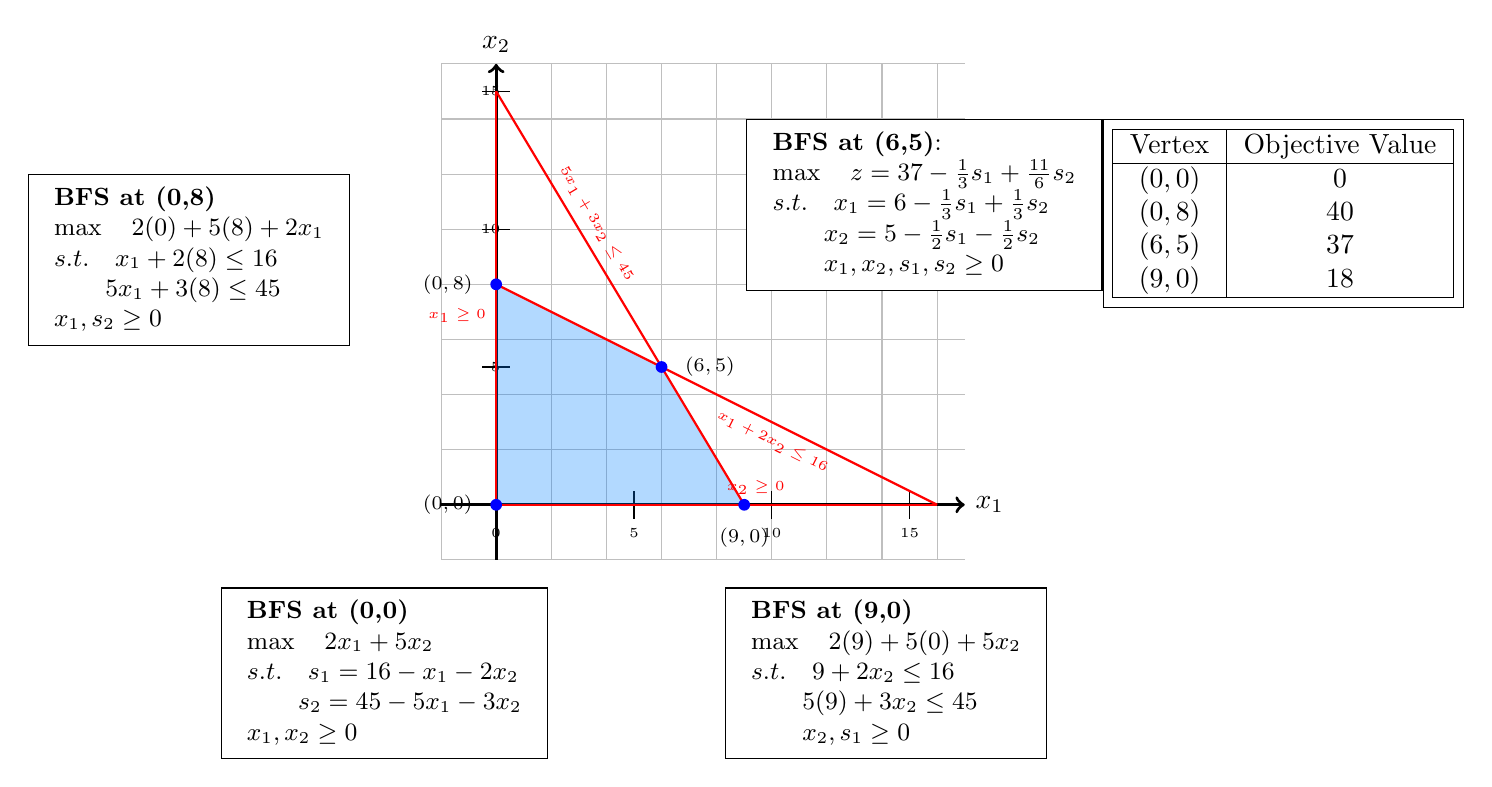
\begin{tikzpicture}[scale = 0.35]
    % Grid and axes
    \draw[gray!50, thin, step=2] (-2,-2) grid (17,16);
    \draw[very thick,->] (-2,0) -- (17,0) node[right] {$x_1$};
    \draw[very thick,->] (0,-2) -- (0,16) node[above] {$x_2$};

    % Axis labels
    \foreach \x in {0,5,10,15} \draw (\x,0.5) -- (\x,-0.5) node[below] {\tiny\x};
    \foreach \y in {0,5,10,15} \draw (-0.5,\y) -- (0.5,\y) node[left] {\tiny\y};

    % Shaded feasible region
    \fill[blue!50!cyan,opacity=0.3] (0,0) -- (0,8) -- (6,5) -- (9,0) -- cycle;

    % Constraint lines
    \draw[red,thick] (0,8) -- node[below right,sloped] {\tiny$x_1 + 2x_2 \leq 16$} (16,0);
    \draw[red,thick] (0,15) -- node[above left,sloped] {\tiny$5x_1 + 3x_2 \leq 45$} (9,0);
    \draw[red,thick] (0,0) -- node[below left] {\tiny$x_1 \geq 0$} (0,15);
    \draw[red,thick] (0,0) -- node[above right] {\tiny$x_2 \geq 0$} (16,0);

    % Vertices
    \node[blue] at (0,0) [circle,fill,inner sep=1.5pt]{};
    \node[blue] at (0,8) [circle,fill,inner sep=1.5pt]{};
    \node[blue] at (6,5) [circle,fill,inner sep=1.5pt]{};
    \node[blue] at (9,0) [circle,fill,inner sep=1.5pt]{};

    % Labels for vertices
    \node[black,anchor=east] at (-0.5,0) {\scriptsize$(0,0)$};
    \node[black,anchor=east] at (-0.5,8) {\scriptsize$(0,8)$};
    \node[black,anchor=west] at (6.5,5) {\scriptsize$(6,5)$};
    \node[black,anchor=north] at (9,-0.5) {\scriptsize$(9,0)$};

    % Optimization problems at each BFS
    \node[draw,fill=white,anchor=north west] at (-10,-3) {
        \small \begin{tabular}{l}
        \textbf{BFS at (0,0)} \\
        \(\max \quad 2x_1 + 5x_2\) \\
        \(\text{s.t. } \quad s_1 = 16 - x_1 - 2x_2\) \\
        \(\quad \quad  s_2 = 45 - 5x_1 - 3x_2\) \\
        \( x_1, x_2 \geq 0 \)
        \end{tabular}
    };

    \node[draw,fill=white,anchor=north west] at (-17,12) {
        \small \begin{tabular}{l}
        \textbf{BFS at (0,8)} \\
        \(\max \quad 2(0) + 5(8) + 2x_1\) \\
        \(\text{s.t. } \quad x_1 + 2(8) \leq 16\) \\
        \(\quad \quad 5x_1 + 3(8) \leq 45\) \\
        \( x_1, s_2 \geq 0 \)
        \end{tabular}
    };

    \node[draw,fill=white,anchor=north east] at (22,14) {
        \small \begin{tabular}{l}
        \textbf{BFS at (6,5)}:\\
        \(\max \quad z = 37 - \frac{1}{3}s_1 + \frac{11}{6}s_2\) \\
        \(\text{s.t. } \quad x_1 = 6 - \frac{1}{3}s_1 + \frac{1}{3}s_2\) \\
        \quad\quad \(x_2 = 5 - \frac{1}{2}s_1 - \frac{1}{2}s_2\)\\
        \quad\quad \( x_1, x_2, s_1, s_2 \geq 0 \)
        \end{tabular}
    };

    \node[draw,fill=white,anchor=north east] at (20,-3) {
        \small \begin{tabular}{l}
        \textbf{BFS at (9,0)} \\
        \(\max \quad 2(9) + 5(0) + 5x_2\) \\
        \(\text{s.t. } \quad 9 + 2x_2 \leq 16\) \\
        \(\quad \quad 5(9) + 3x_2 \leq 45\) \\
      \quad \quad  \( x_2, s_1 \geq 0 \)
        \end{tabular}
    };

    % Table within the TikZ picture
    \node[draw,fill=white,anchor=north west] at (22,14) {
        \begin{tabular}{|c|c|}
        \hline
        Vertex & Objective Value \\
        \hline
        $(0,0)$ & $0$ \\
        $(0,8)$ & $40$ \\
        $(6,5)$ & $37$ \\
        $(9,0)$ & $18$ \\
        \hline
        \end{tabular}
    };

\end{tikzpicture}
\end{center}
\caption{\href{https://www.desmos.com/calculator/j1li4l7lcv}{Desmos: Interactive plot!} (\href{https://open-optimization.github.io/open-optimization-or-book/Intro-Math-Programming/baseText/interactive-figures/lp-graphical-method.html}{backup interactive plot}) Showing the optimization problem from different BFS perspectives.}
\end{figure}

